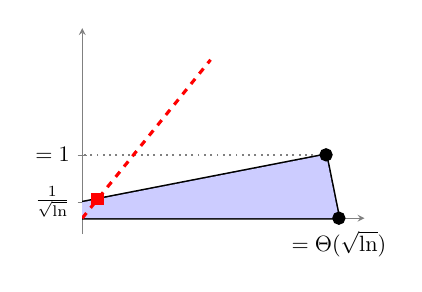
\begin{tikzpicture}[scale=0.8, transform shape]
\begin{axis}[
axis line style=gray,
axis lines=middle,
xlabel = $\buyerexanteutil$,
ylabel = $\sellerexanteutil$,
xtick={0, 1},
ytick={0, 0.1, 0.4},
xticklabels={0, $\buyerbenchmark=\Theta(\sqrt{\ln\constantH})$},
yticklabels={0, $\frac{1}{\sqrt{\ln\constantH}}$, $\sellerbenchmark = 1$},
xmin=0,xmax=1.1,ymin=-0.1,ymax=1.2,
width=0.5\textwidth,
height=0.4\textwidth,
samples=1000]


\addplot[black!100!white, line width=0.5mm] (0, 0) -- (0, 0.1) -- (0.95, 0.4) -- (1, 0) -- (0, 0);

\fill[blue!20] (0, 0) -- (0, 0.1) -- (0.95, 0.4) -- (1, 0) -- (0, 0);



\addplot[dotted, gray, line width=0.3mm] (0.9, 0.4) -- (0, 0.4);

\addplot[dashed, red, line width = 0.5mm] (0, 0) -- (0.5, 1);

\draw[black, fill=black, line width=0.5mm] (axis cs:1, 0) circle[radius=0.08cm];
\draw[black, fill=black, line width=0.5mm] (axis cs:0.95, 0.4) circle[radius=0.08cm];

% \draw[red, fill=red, line width=0.5mm] (axis cs:0.06, 0.12) circle[radius=0.08cm];

\draw[red, fill=red, line width=0.5mm] (0.04, 0.09) rectangle (0.08, 0.15);

\end{axis}

\end{tikzpicture}